\documentclass[border=2mm]{standalone}

\usepackage{tikz}
\usepackage[american,smartlabels,fulldiodes,siunitx]{circuitikz}
\usetikzlibrary{calc}
\usetikzlibrary{shadows}
\usetikzlibrary{arrows.meta}

\ctikzset{bipoles/thickness=1}
\ctikzset{bipoles/length=0.8cm}
\ctikzset{bipoles/diode/height=.375}
\ctikzset{bipoles/diode/width=.3}
\tikzstyle{every node}=[font=\small]
\tikzstyle{every path}=[line width=0.8pt,line cap=round,line join=round]

\newcommand{\dcdc}[2]{
	\node at ($#1+(0.15,0.3)$) (#2_in1) {};
	\node at ($#1+(-0.15,0.3)$) (#2_in2) {};
	\node at ($#1+(0,0.3)$) (#2_in3) {};
	\node at ($#1+(-0.15,-0.3)$) (#2_out1) {};
	\node at ($#1+(0,-0.3)$) (#2_out3) {};
	\node at ($#1+(0.15,-0.3)$) (#2_out2) {};
	\draw[fill=white,drop shadow] ($#1+(-0.3,-0.3)$) rectangle ($#1+(0.3,0.3)$);
	\draw ($#1+(-0.3,-0.3)$) -- ($#1+(0.3,0.3)$);
	\node at ($#1+(-0.1,0.2)$) () {\tiny DC};
	\node at ($#1+(0.1,-0.2)$) () {\tiny DC};
}

\begin{document}
	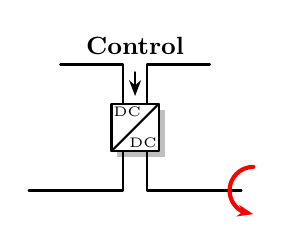
\begin{tikzpicture}
		\tikzstyle{arrow} = [-{Stealth[length=1.2mm, width=1mm]}]
		
		\node at (0,0) (conv) {};
		\dcdc{(conv)}{C};
		
		\draw (C_in2.base) to[short] +(0,0.5) to[short] +(-0.8,0.5);
		\draw (C_in1.base) to[short] +(0,0.5) to[short] +(0.8,0.5);
		
		\draw (C_out1.base) to[short] +(0,-0.5) to[short] +(-1.2,-0.5);
		\draw (C_out2.base) to[short] +(0,-0.5) to[short] +(1.2,-0.5);
		
		\draw[red,line width=1.5pt] (1.2,-0.8) arc[start angle=180, end angle=90, radius=0.3];
		\draw[red,-{Stealth[length=2mm, width=1.5mm]},line width=1.5pt] (1.2,-0.8) arc[start angle=180, end angle=270, radius=0.3];
		
		\node[anchor=south] at (0,0.8) {\textbf{Control}};
		\draw[-{Stealth[length=2mm, width=1.5mm]},line width=1pt] (0,0.7) -- (0,0.4);
		
	\end{tikzpicture}
\end{document}
